\section{Autocrop Results}

For the improved auto cropping mechanism there are many different versions implemented in this work.
All of them have been evaluated on the Switch evaluation dataset.
Even though the cropping mechanism is primarily designed for the inference of videos, performance differences can be recorded in this dataset.
The track of each image is predicted 50 times and the crop coordinates are adjusted iteratively.
The Results of autocrop versions are shown in \autoref{tab:autocropResults}.

\begin{table}[H]
    \centering
    \begin{tabular}{|l|c|c|c|c|c|}
    %\begin{tabular}{| p{0.3\linewidth} | p{0.6\linewidth} |}
        \hline
        \textbf{used Methods} & \textbf{original \cite{tepNet2024}} & \textbf{Version 2} & \textbf{Version 3} & \textbf{Version 4} & \textbf{Version 5}\\
        \hline
        RA                                 & \checkmark &            &            &            &            \\
        \hline
        EMA                                &            & \checkmark & \checkmark & \checkmark & \checkmark \\
        \hline
        reset rule [40\%] $(\frac{1}{3}, \frac{1}{2}, \frac{2}{3})$  &            & \checkmark & \checkmark & \checkmark & \checkmark \\
        \hline
        aspect ratio (16:9)   	           &            &            & \checkmark &            &            \\
        \hline
        aspect ratio (1:1)                 &            &            &            & \checkmark &            \\
        \hline
        10\% at the start                  &            &            &            &            & \checkmark \\
        \hline
        Switch evaluation dataset          & 88.97\%    & \textbf{91.18\%} & 86.76\% & 91.18\% & 90.44\%    \\
        \hline
    \end{tabular}
    \caption{Various versions of autocrops evaluated on the Switch evaluation dataset.
    Models predict each image 50 times and adjust the autocrop iteratively.
    Version 2 includes multiple experiments different parameters for the reset rule.
    Since the Evalutation dataset consists of images and the reset rule is applied in video sequences, only the best-performing parameters are included in this table.}
    \label{tab:autocropResults}
\end{table}

An improvement in accuracy can be observed in all versions but version 3.
In Version 3, the crop is forced to be in a 16:9 aspect ratio.
It is assumed that this ratio presents a disadvantage since the crop is resized in a quadratic 512 $\times$ 512 image afterward.
This assumption is supported by Version 4 also achieving the highest score.
This version has a fixed quadratic aspect ratio.

Version 5 is very similar to Version 2 but instead of starting with the whole image, its initial crop coordinates are set to $(0, 0.1 \times image\_height, 1)$.
The whole image width but only the lowest 10\% of the image are considered.
This proves to be effective in some cases, resulting in a much quicker convergence to a desired crop.
However, it also shows that it is highly situational dependent.
Version 5 works better than starting with the whole image only when a single track is visible in the beginning.
In starting scenarios with at least two tracks the model struggles to find the right one. Therefore the use of Version 5 is not recommended.
Version 2 and 4 are the highest-performing methods.
However, for this work Version 2 is used for further experiments because it does not introduce additional heuristics like Version 4.
Therefore, it is more independent of scene situations.

The parameters of the reset rule are chosen according to the behavior of models in different situations.
In uncertainty, all Models have receding horizon lines, even though different backbones are used.
Therefore the crop is reset when the prediction is below 40\% of the crop height.
Thresholds of 30\% 40\%, 50\%, and 60\% are tested.
With 50\% and 60\%, the crop is sometimes reset even though the prediction is correct, and with 30\% the convergence takes too much time.
Therefore 40\% is chosen to be the threshold.
The crop is reset to $(\frac{1}{3}, \frac{1}{2}, \frac{2}{3})$.
These parameters are near the optimal crop coordinates for all test scenarios without narrowing the crop too much, which would lead to a possible collapse.

\vspace{1cm}

To qualitatively show the difference between the original auto crop from \cite{tepNet2024} and the proposed one for this work, both are tested on a difficult scenario.
A video from a train driving through a railroad station with many rails, switches, and crossings is chosen to evaluate the different auto-crop mechanisms to their cores.
Additionally, the ResNet18 backbone is used because it is the worst-performing one in terms of accuracy and differences can be observed more easily.


\begin{figure}[H]
    \centering

    % Unteres Grid mit kleineren Bildern
    \begin{minipage}{0.195\textwidth}
        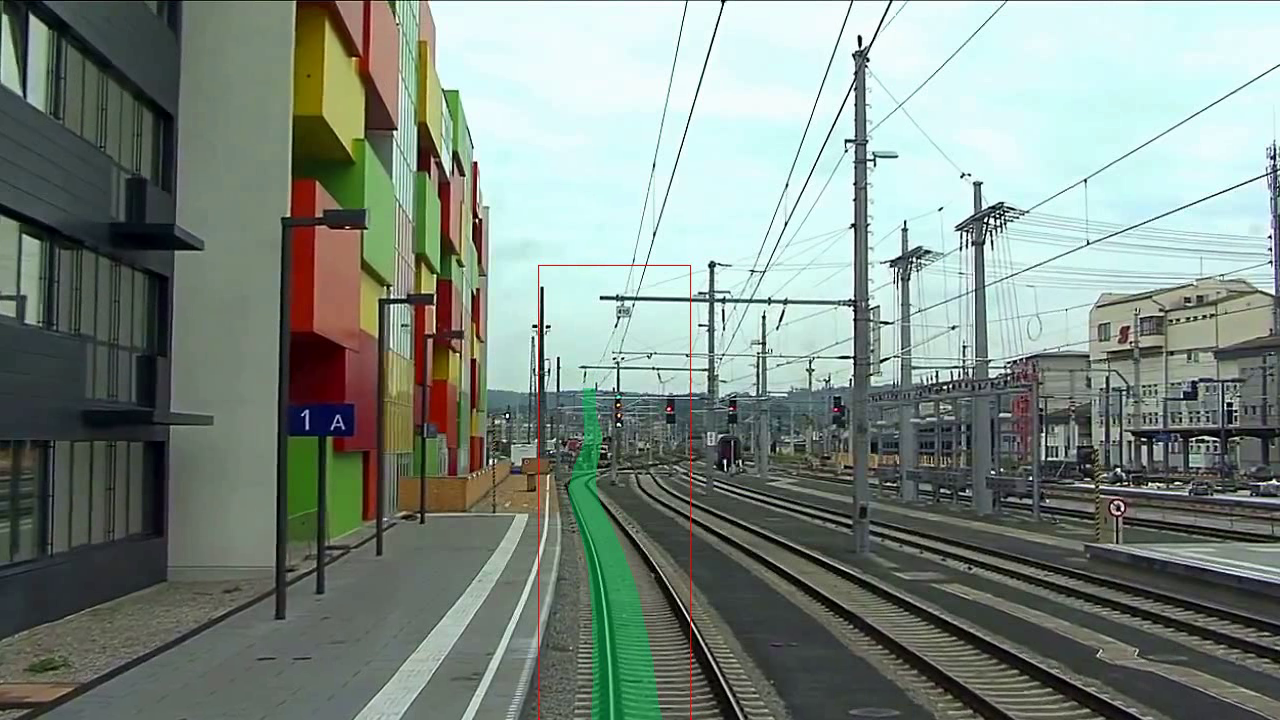
\includegraphics[width=\textwidth]{PICs/experiments/autocropExperiments/output_frames/frame_100.png}
    \end{minipage}
    \hfill
    \begin{minipage}{0.195\textwidth}
        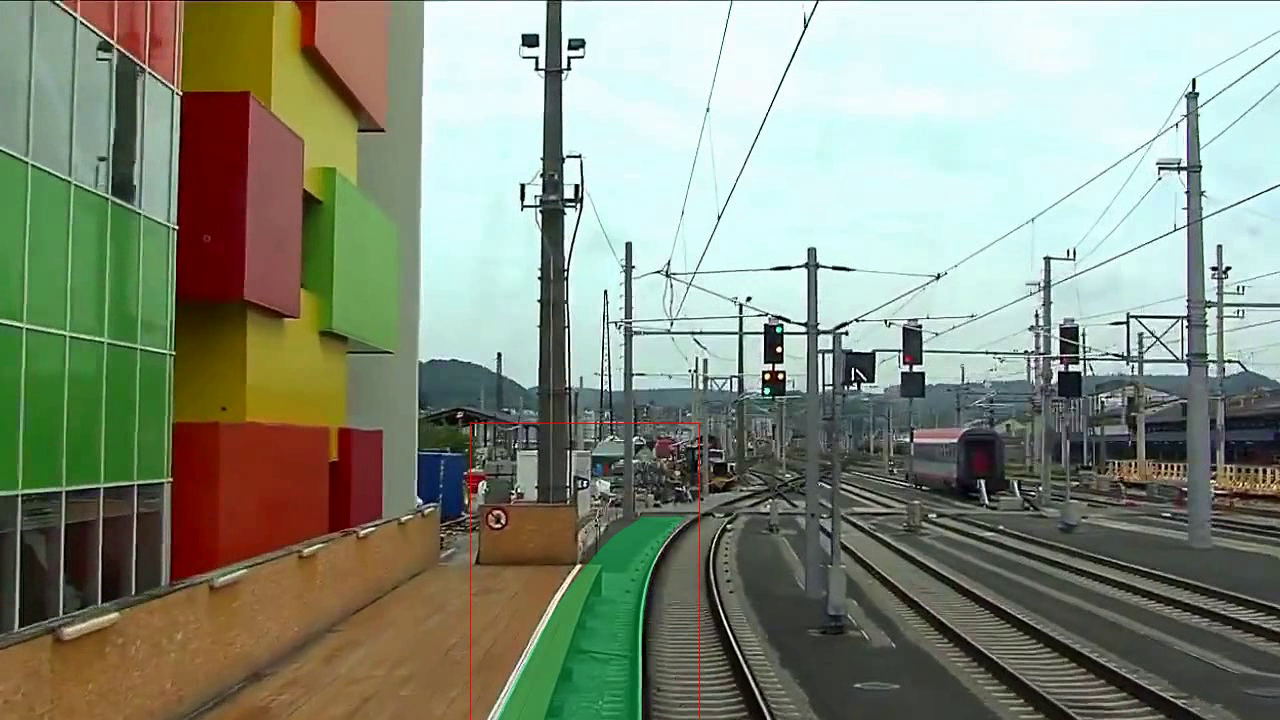
\includegraphics[width=\textwidth]{PICs/experiments/autocropExperiments/output_frames/frame_700.png}
    \end{minipage}
    \hfill
    \begin{minipage}{0.195\textwidth}
        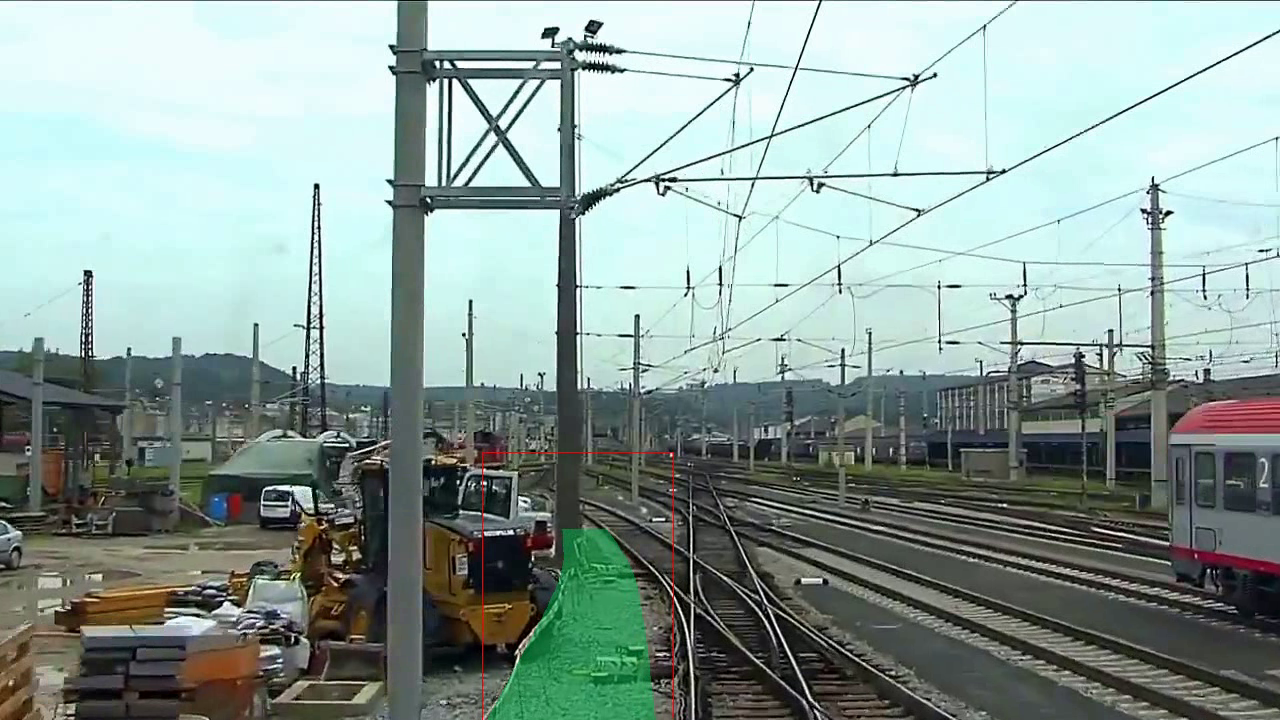
\includegraphics[width=\textwidth]{PICs/experiments/autocropExperiments/output_frames/frame_1000.png}
    \end{minipage}
    \hfill
    \begin{minipage}{0.195\textwidth}
        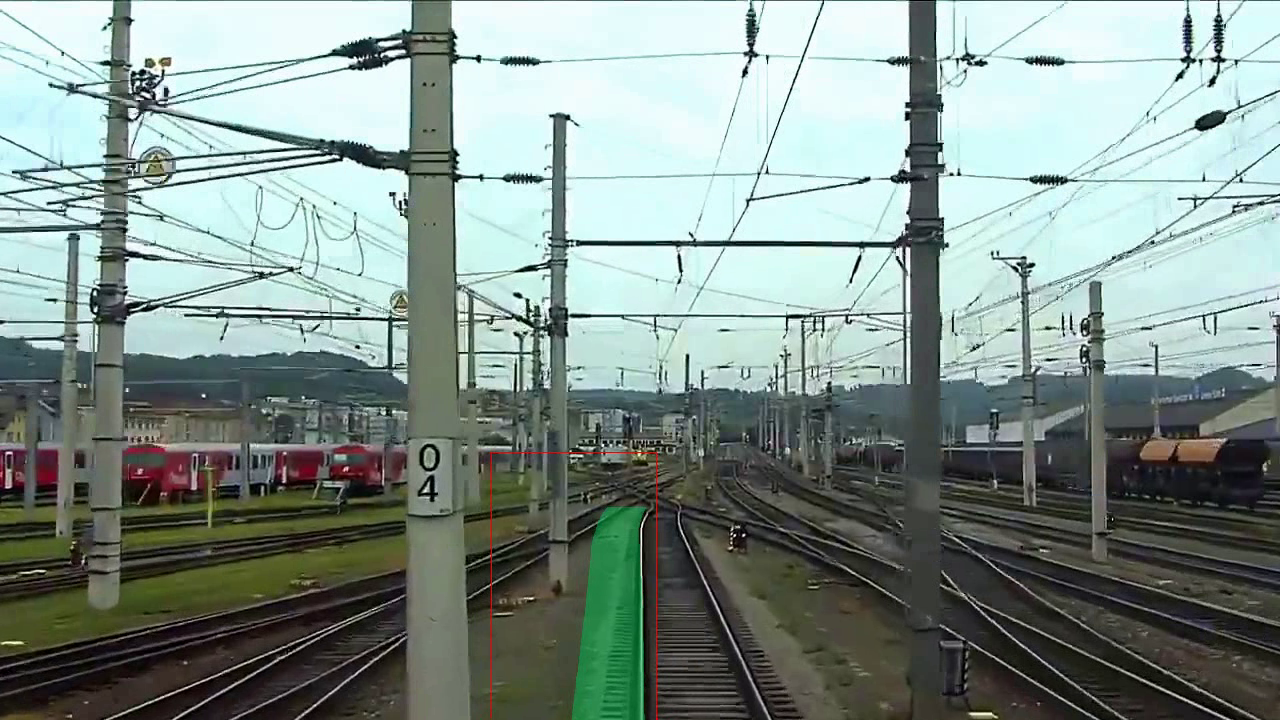
\includegraphics[width=\textwidth]{PICs/experiments/autocropExperiments/output_frames/frame_1600.png}
    \end{minipage}
    \hfill
    \begin{minipage}{0.195\textwidth}
        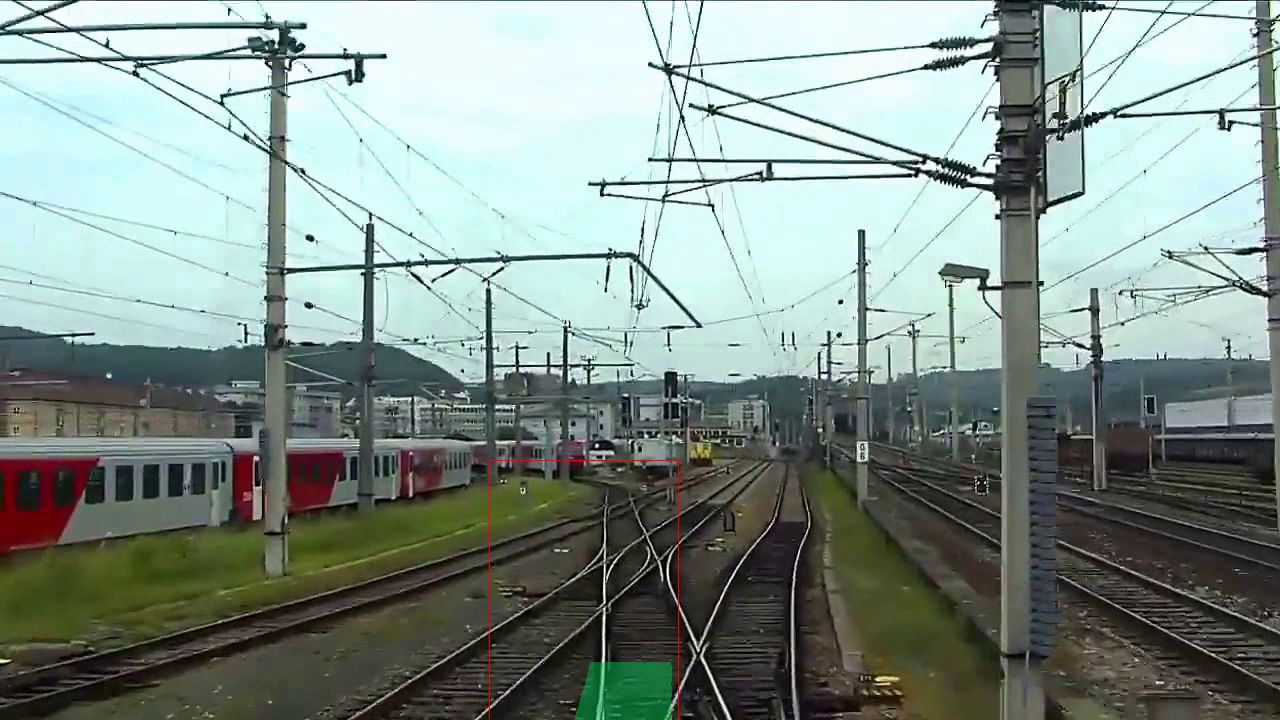
\includegraphics[width=\textwidth]{PICs/experiments/autocropExperiments/output_frames/frame_1900.png}
    \end{minipage}

    % Unteres Grid mit kleineren Bildern
    \begin{minipage}{0.195\textwidth}
        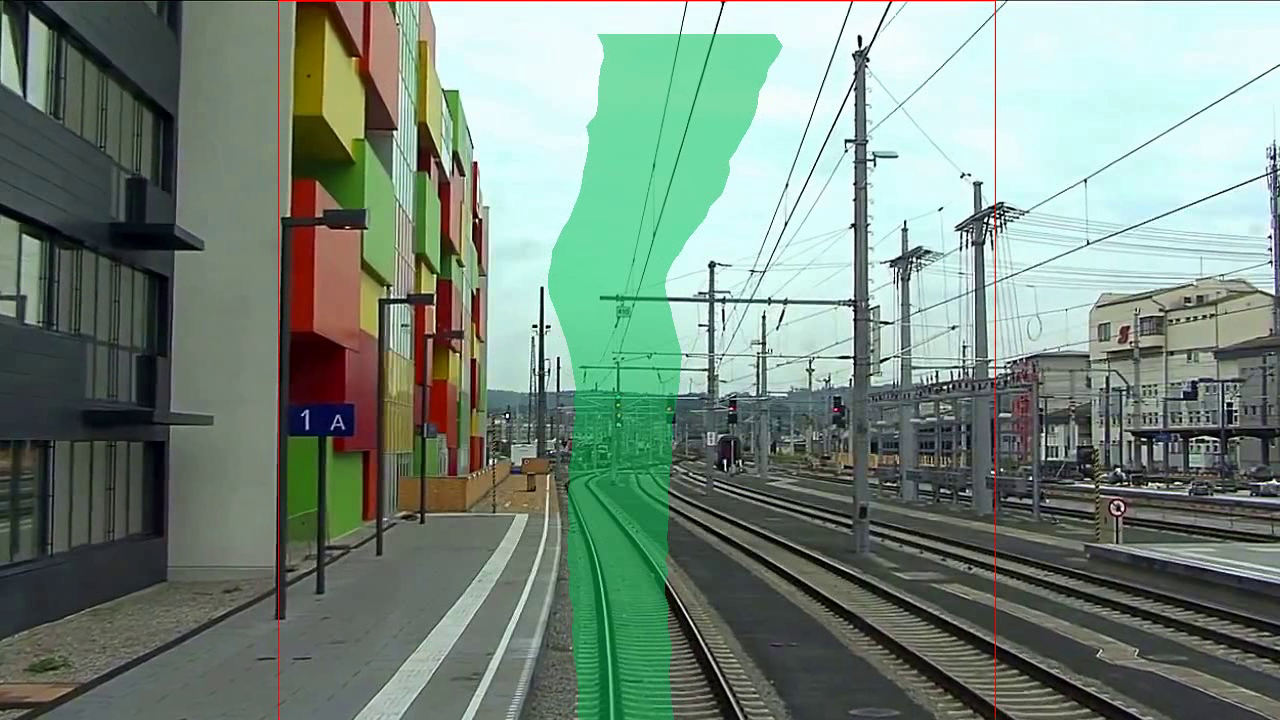
\includegraphics[width=\textwidth]{PICs/experiments/autocropExperiments/output_frames_improved/frame_100.png}
    \end{minipage}
    \hfill
    \begin{minipage}{0.195\textwidth}
        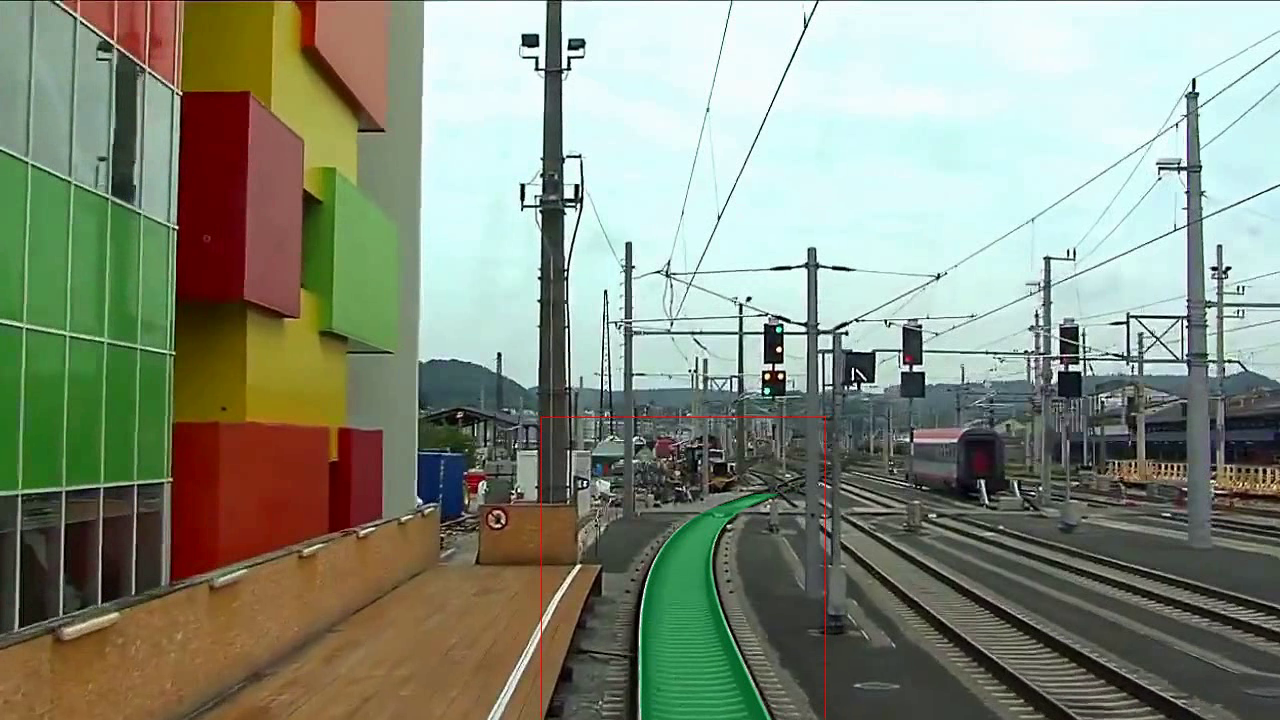
\includegraphics[width=\textwidth]{PICs/experiments/autocropExperiments/output_frames_improved/frame_700.png}
    \end{minipage}
    \hfill
    \begin{minipage}{0.195\textwidth}
        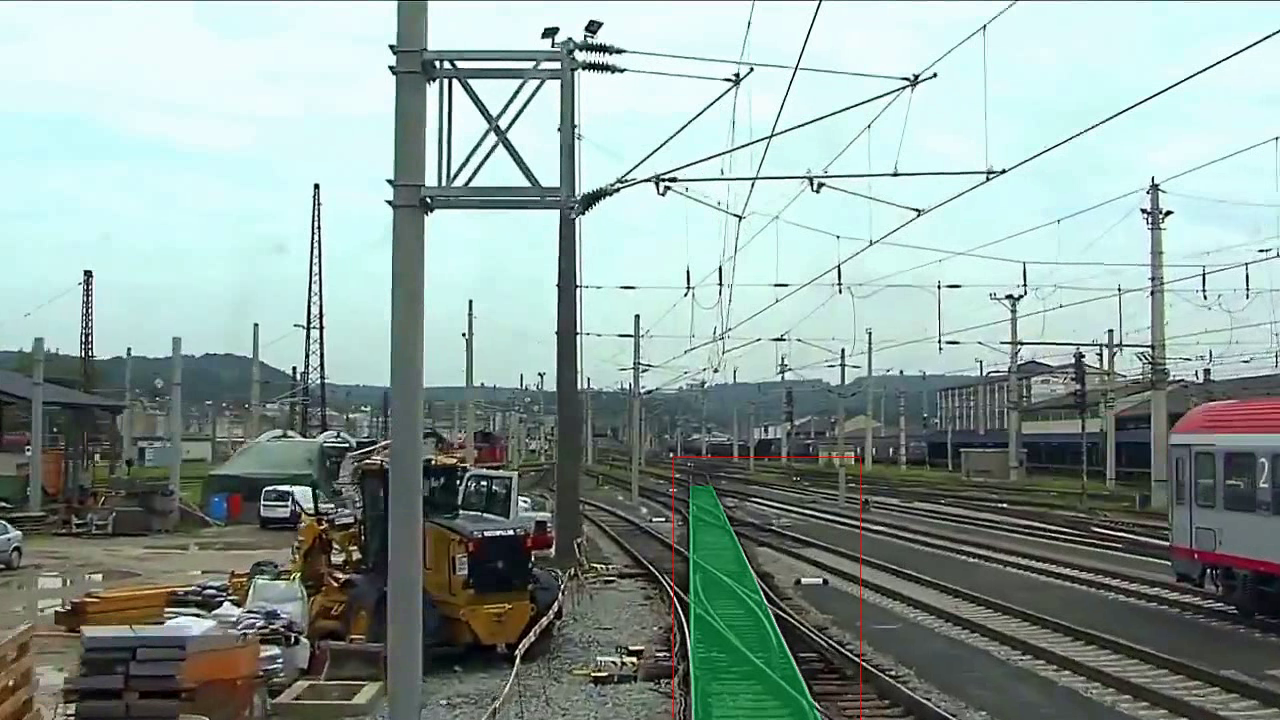
\includegraphics[width=\textwidth]{PICs/experiments/autocropExperiments/output_frames_improved/frame_1000.png}
    \end{minipage}
    \hfill
    \begin{minipage}{0.195\textwidth}
        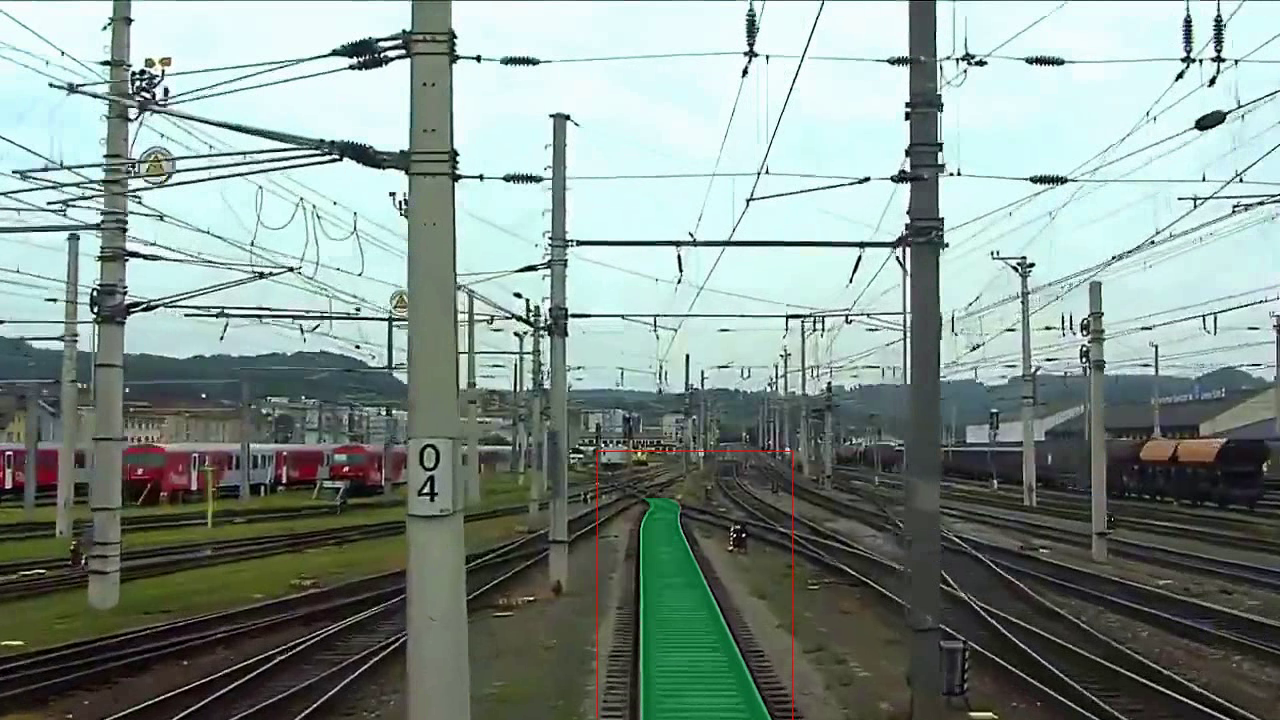
\includegraphics[width=\textwidth]{PICs/experiments/autocropExperiments/output_frames_improved/frame_1600.png}
    \end{minipage}
    \hfill
    \begin{minipage}{0.195\textwidth}
        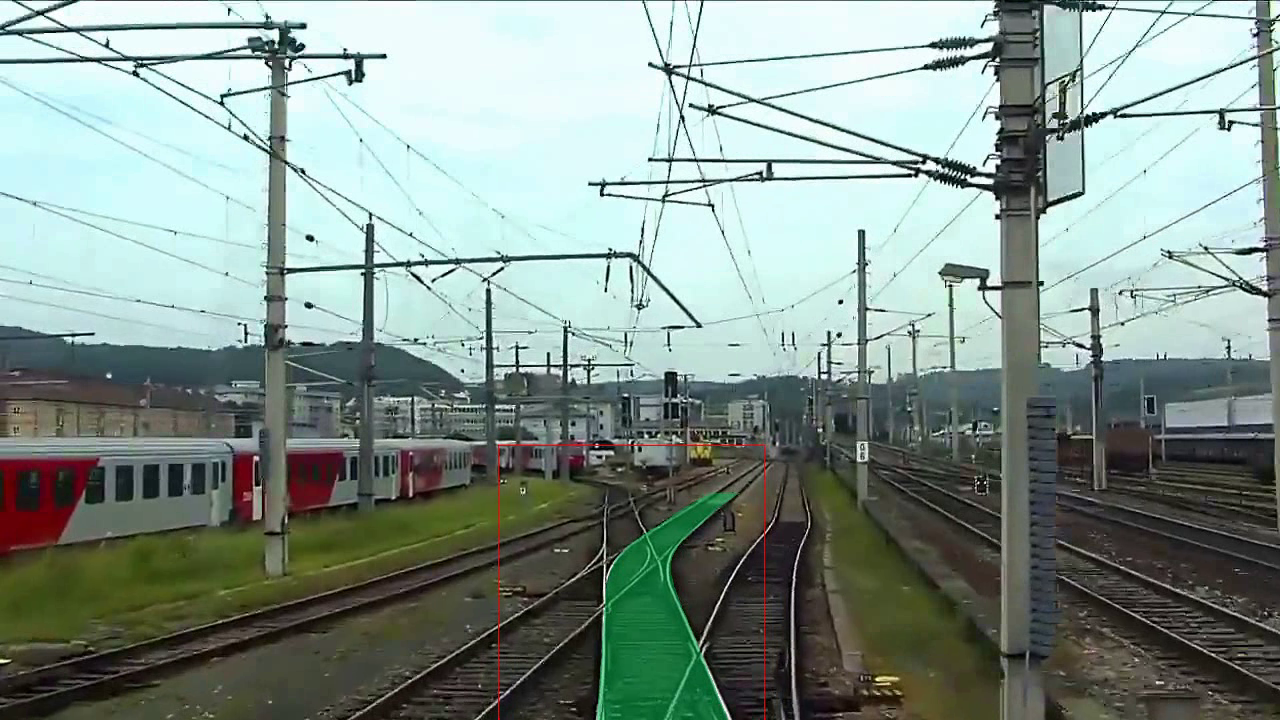
\includegraphics[width=\textwidth]{PICs/experiments/autocropExperiments/output_frames_improved/frame_1900.png}
    \end{minipage}

    % Vierte Reihe für die Zeitachse
    \begin{minipage}{1.0\textwidth}
        \centering
        \begin{tikzpicture}
            % Zeit "Time" über dem Pfeil links positionieren
            \node at (-7.5, 0.3) {time}; % Text "Time"
            \draw[-Stealth, thick] (-8, 0) -- (8, 0); % Pfeil von ganz links nach ganz rechts
        \end{tikzpicture}
    \end{minipage}

    % Beschriftung unter dem Grid
    \vspace{0.5cm}
    \caption{Autocrop video comparison}
    \label{fig:autocropVideoComparison}
\end{figure}


\begin{figure}[H]
    \centering
    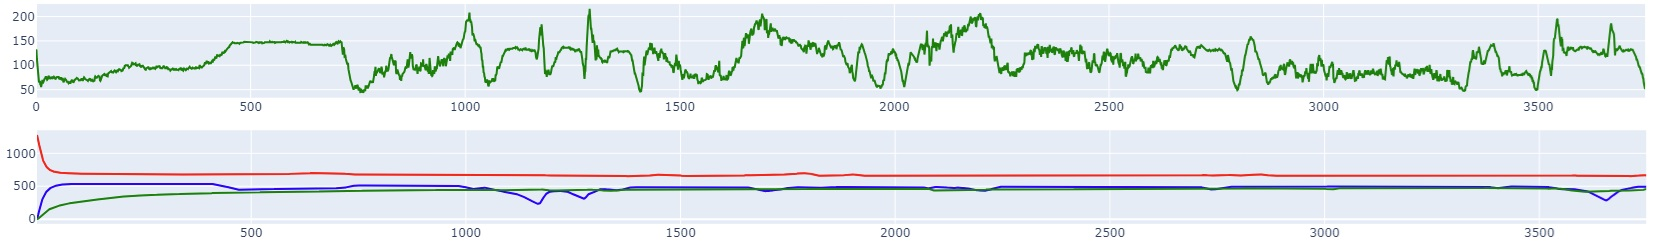
\includegraphics[width=\textwidth]{PICs/experiments/autocropExperiments/original.jpg} % erstes Bild
    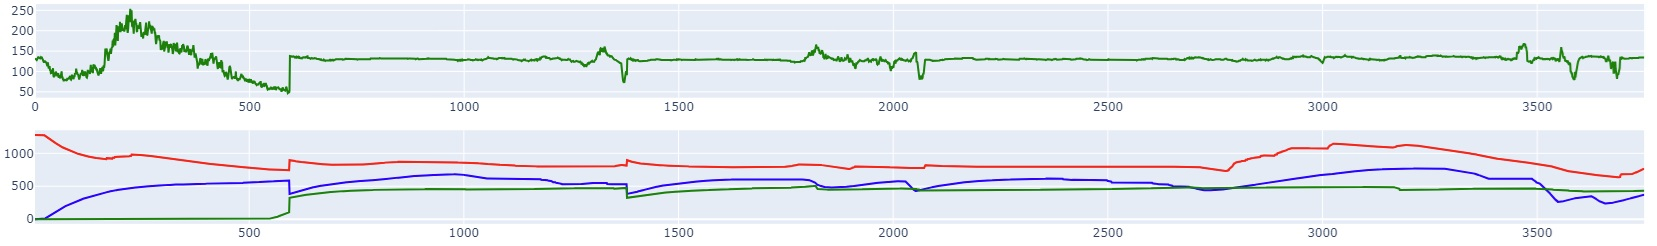
\includegraphics[width=\textwidth]{PICs/experiments/autocropExperiments/improved.jpg} % zweites Bild
\end{figure}